\chapter{Medical Fundamentals}
Comprehension of the physiological functionality of the human heart and the cardiovascular system is an important prerequisite to the work addressed in this thesis. Therefore the basics of these topics will be explained in this chapter.

\section{Cardiovascular System}
The fundamental task of the cardiovascular system is to supply all organs with blood. The system, is divided into two components. The systemic circulation and the pulmonary circulation. As shown in Figure \ref{fig:circulation}, which represents the percentage distribution of the blood over the circulatory system, the systemic circulation is supplying blood flow to all tissues and organs except the lung. Due to this it is also referred to as the greater circulation. \cite{GH20}
\begin{figure}[h]
  \centering
  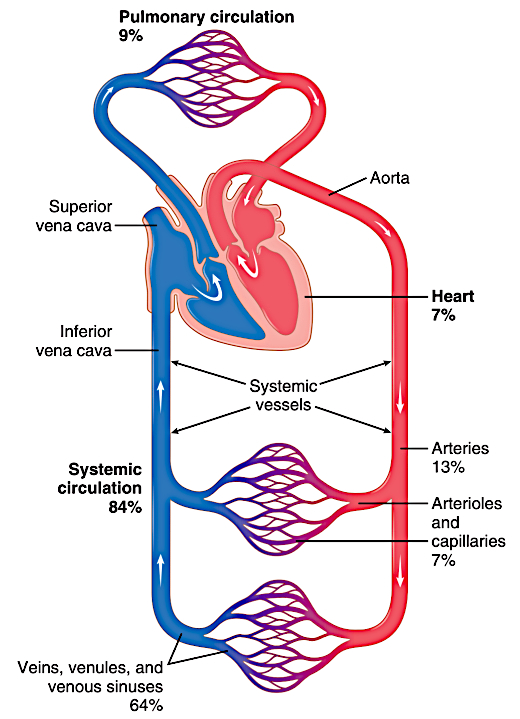
\includegraphics[width=0.4\textwidth, height=0.6\textwidth]{images/circulation.jpg}
  \caption{Blood distribution in circulatory system \cite{GH20}}
  \label{fig:circulation}
\end{figure}
 The center of the circulatory system is the heart. The heart itself consists of two mechanical pumps, which are functionally connected in series, but are united in one organ. It is seperated into two sides, which themselfs are divided into an atrium and a ventricle. The atria act as weak primer pumps, needed to provide blood flow to the ventricles.\cite{HKS4} Both the atrium and the ventricle are surrounded by the myocardium, which acts as the working muscle of the heart. Through the contraction of the myocardium blood is pumped into the circulatory system.\cite{HKS7} This contraction is actuated by an electrical action potential originating from the sinus node. The left ventricle is pumping oxygenated blood through the aorta into the systemic circulation. There, the oxygen stored in the blood is delivered to the organs. The blood, now low in oxygen, is then led into the right atrium through the inferior and superior vena cava. From the right atrium, the deoxygenated blood then enters the right ventricle and then the pulmonary circulation via the pulmonary artery. After the blood is oxygenated in the lungs, it is returned to the left atrium through the pulmonary vein.\cite{HKS4} Figure \ref{fig:heart_anat} provides a graphic overview on the anatomy of the heart and the course of blood flow through the heart.
\begin{figure}[h]
  \centering
  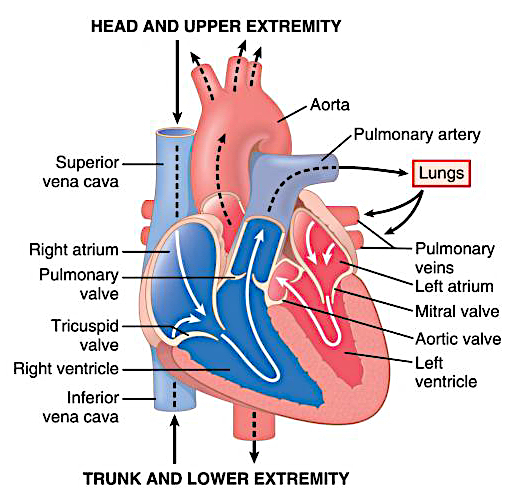
\includegraphics[width=0.6\textwidth]{images/heart_1.jpg}
  \caption{Anatomy of the heart \cite{GH20}}
  \label{fig:heart_anat}
\end{figure}
\\The process of contraction of the heart, also called the cardiac cycle, is divided into 4 phases.

\begin{figure}[h]
  \centering
  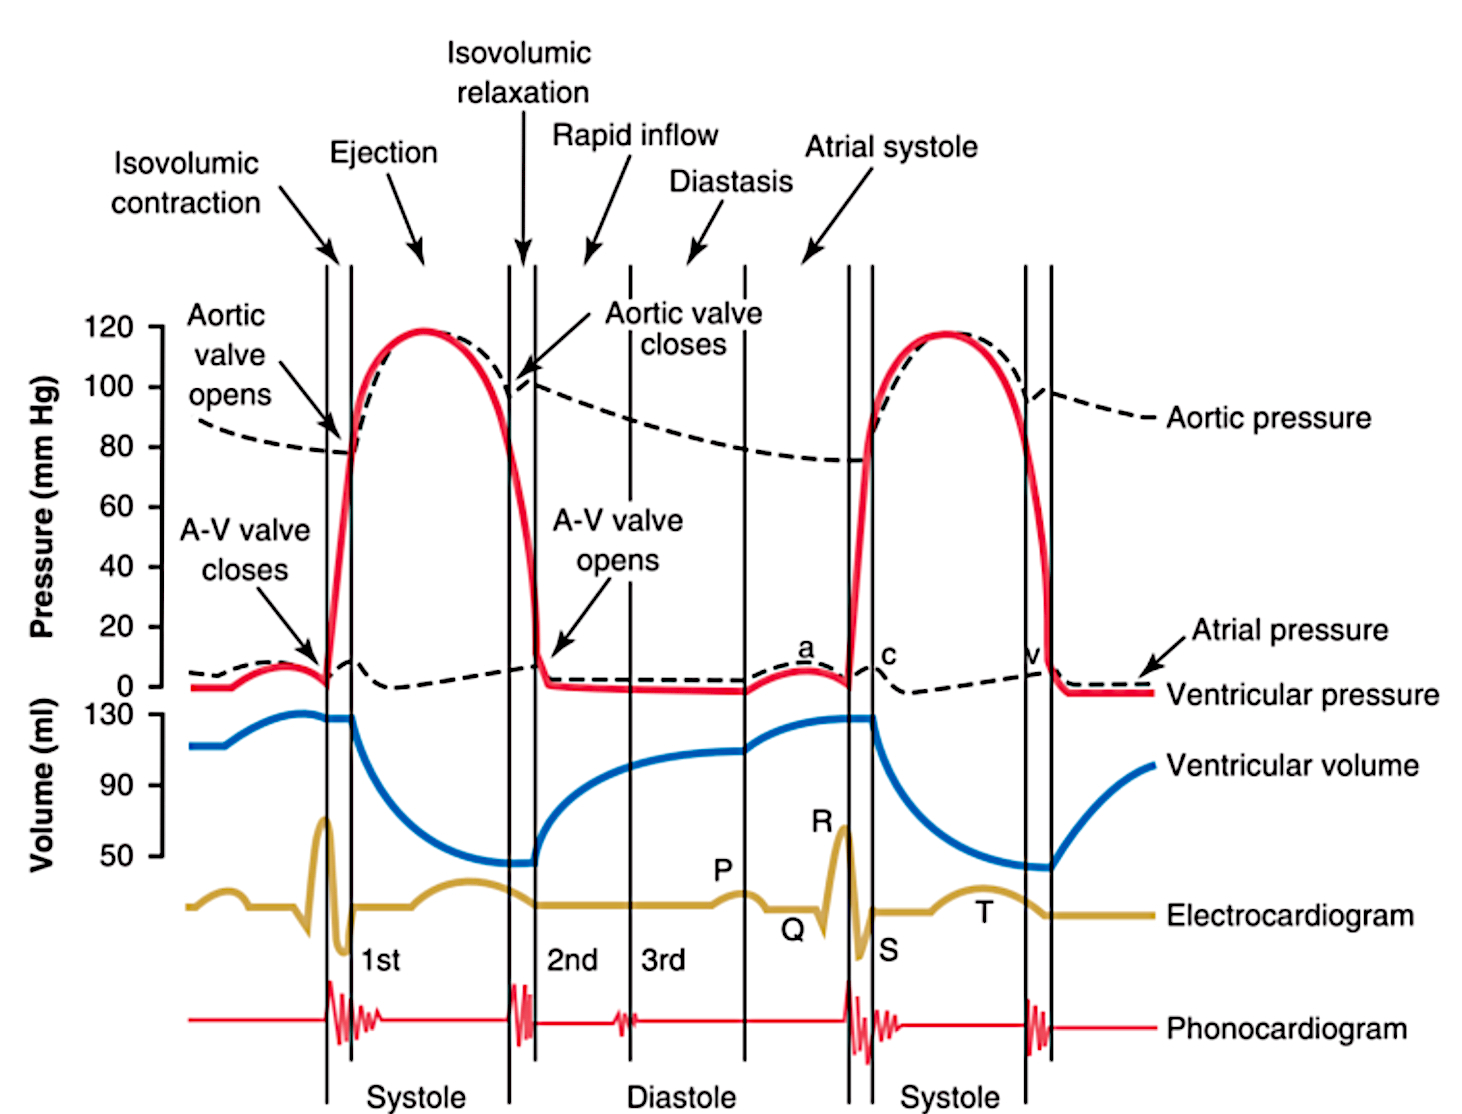
\includegraphics[width=0.8\textwidth]{images/cardiac_cycle.jpg}
  \caption{Action phases of the cardiac cycle based on the example of the left ventricle \cite{GH20}}
  \label{fig:cardiac_cycle}
\end{figure}
\section{Heartinsufficency}
